\section{Errors and Sensitivity}


The anticipated statistical errors, including the error from azimuthal fitting of the data, are shown in Fig. \ref{cpp_theory_fit}.
The errors assume 20 days of running on a 5 \% radiation length $^{116}$Sn target, 10$^7$ photons/s, and nominal acceptance for $\pi^+ \pi^-$.
Table \ref{errors} summarizes the estimated statistical and systematic errors. In the following we describe each of
these contributions in detail: 

%\end{landscape}
% \begin{landscape}
\begin{table}[bt]
\caption{Statistical errors, correction factors, and uncertainties in correction factors.
\label{errors}
}
\begin{center}
\begin{tabular}{|l|c|c|c|c|c|c|c|c|}
\hline
\hline
    Errors and correction factors  &  Correction       & Statistical uncertainty    \\ 
                                                         &     factor            & in correction factor    \\  \hline \hline
  Overall statistical error  &      &  0.6 \%    \\ \hline
  Normalization to $\mu^+ \mu^-$  and relative trigger efficiency &     &  1 \%     \\ \hline
  $\mu^+ \mu^-$ background in $\pi^+ \pi^-$ yield  & 0.03 \% &  0 \%   \\ \hline
%  Relative acceptance  & ?? & ??  \\ \hline
  Polarization  &   70\%   &  0.2 \%     \\ \hline
  Pion identified as muon, and pion decay &  8 \%   &   1\%   \\ \hline
  Total systematic error &   & 1.5 \% \\ \hline
  Projected error in $\alpha - \beta$ &   &  10\%  \\ \hline
 \hline
 \hline
\end{tabular}
\end{center}
\end{table}
%\end{landscape}

\begin{enumerate}

\item
Overall statistical error:  This aggregate error is based on fitting the $\phi_{\pi \pi}$ distribution to
extract the Primakoff yield, and then fitting a theoretical curve to the W$_{\pi \pi}$ data points (see figures \ref{sample_phi_psi_fit}-\ref{cpp_theory_fit}).

\item
Normalization to $\mu^+ \mu^-$ and relative trigger efficiency: 
This is the estimated uncertainty for a calculation of $\gamma A \rightarrow \mu^+ \mu^- A$%, and the effect
of uncertainties in the relative trigger efficiences of pions versus muons, 1 \%.  

\item
$\mu+ \mu^-$ background in $\pi^+ \pi^-$ yield: The background considered  here is the case where a muon fails to trigger the
muon detector behind the iron shield.  If we assume the muon chamber has x, u, v planes with 95\% plane efficiency for minimum ionizing particles, then
the overall chamber efficiency is 99.3\%. Assuming
a 5:1 muon:pion ratio, then the probability for both tracks failing to trigger the muon counter is very small, 0.03\%.
The efficiency of the muon counter can be measured by examining events in kinematics where muon pair production dominates, where one track tags as
a muon, then  measuring the  probability for the second track to tag as a pion.

%\item
%Relative acceptance. The measured rates for muon and pion pairs depends on the acceptance at small angles, approximately 0.8$^o$. 
%As the Primakoff cross section will be determined relative to muon pair production, an uncertainty is introduced because the
%acceptance for the two processes are not quite the same. The acceptance change for the Primakoff signal over the 2$\sigma_{\theta}$=0.14$^o$,
%is .....\%, while the muon production changes by .....\%. The relative acceptance changes by...\%. 


\item
Polarization: The photon polarization is determined by measuring the azimuthal distribution of (i) $\mu^+ \mu^-$ pairs, and
(ii) $\pi^0$ from coherent photo-production.  Since there are approximately five times as many $\mu^+ \mu^-$ pairs in the data
as compared to $\pi^+ \pi^-$, the statistical precision will be very high in this method, approximately 0.2 \%.  The purity of the $\mu^+ \mu^-$
sample will not be a limiting factor. Pion contamination can be estimated by assuming
 5 hadronic interaction lengths for FCAL + iron absorber, then the  probability for a pion
to punch through is approximately 0.7 \%. The probability for both pions to punch through,  weighted by the 1:5 pion:muon ratio, is
negligible. Pions can also register as muons through pion decay (see discussion below for ``One or both pions decays in flight'').  
Taking the worst case that
all 4 \% of the pions that decay will be tagged as muons, gives a pion contamination in the muon yield of 0.03 \%.


\begin{figure}[th]
\centering
%\includegraphics[width=4in]{figures/sample_phi_psi_fit.pdf}
\caption{Example fits of the $\phi_{\pi\pi}$ spectrum (top, red) and the $\psi_{\pi\pi}$ spectrum (bottom, blue) for the $W_{\pi\pi}$ bin centered at $330 MeV/c^2$. The polarization was fixed at 70\% (corresponding to the generated data set). The one free parameter of the fit gave either the fraction of Primakoff (top) or $\rho^{o}$ (bottom) events. The angles used here are from generated values, but with a cut on $\theta>0.8^{\circ}$ to represent the acceptance of the detector.}
\label{sample_phi_psi_fit}
\end{figure}

\begin{figure}[tp]
\centering
%\includegraphics[width=5in]{figures/Wpipi_fit.pdf}
\caption{Results of all fits similar to those shown in Figure \ref{sample_phi_psi_fit}. The fractions obtained from the $\phi_{\pi\pi}$($\psi_{\pi\pi}$) dependent fits are used to calculate the number of Primakoff($\rho^{o}$) events in each $W_{\pi\pi}$ bin. The red(blue) markers indicate the extracted number of events of each type in the bin and the magenta squares are the sums of the red and blue points in each bin. Values used here are generated, but with a cut on $\theta>0.8^{\circ}$ to represent the acceptance of the detector. }
\label{Wpipi_fit}
\end{figure}


\item
Pion identified as muon, and pion decay: These issues are linked, through pion decay, 
and require a unified calibration treatment using simulation and data analysis. 
To limit the uncertainty in correcting the data  we expect that it will be necessary
to carefully simulate pion decay in the experiment, and calibrate the simulation relative to experimental data. Calibration data might be taken in a kinematic regime where $\gamma A \rightarrow \rho^0 A$ dominates over muon pair production by several orders of magnitude. 
We are developing a detailed simulation of the experimental setup to study the effects of pion decay. 
The overall correction factor for these effects will be approximately 8 \%.  We believe that by careful simulation, and calibration of 
the simulation to experimental data, the uncertainty in this correction factor can be limited to $\approx 1 \% $.  


\item
Total systematic error: Combining the systematic errors in quadrature gives 1.5\%.

\item
Projected error in $\alpha - \beta$: Combining the statistical and systematic errors in quadrature,  and using the approximate sensitivity of the
cross sections to $\alpha - \beta$, ($\Delta(\alpha - \beta)/\Delta \sigma = 130\% /20\%$ ), gives an estimated error of 10 \%.  The absolute 
error in $\alpha -\beta$ is therefore $\pm 0.6 \times 10^{-4} fm^3$ . 

\end{enumerate}

\begin{figure}[tp]
\centering
%\includegraphics[width=5in]{figures/cpp_theory_fit.pdf}
\caption{Theory curves for two predicted values of $\alpha_{\pi}-\beta_{\pi}$, the dashed
curve is for 5.7 (ChPT), the dotted curve is for 13.0 (Fil'kov). 
The black points are published data from the MARK-II measurement. 
The red points indicate the anticipated statistical errors for the proposed measurement.
Error bars are taken from those for the Primakoff fits (red) in Figure \ref{Wpipi_fit}.}
\label{cpp_theory_fit}
\end{figure}

\clearpage

\section{Summary and beam request}

Table \ref{request} summarizes the beam request and experimental requirements for the measurement.  20 days are requested for
data production, which  will allow the statistical error to be reasonably below the projected systematic
error, 0.6\,\% versus 1.5\,\%.  The are several non-standard installations required for the running of the
experiment: (1) the liquid hydrogen target will be  removed, and a solid target installed near the upstream
entrance of the magnet, (ii) the muon system will be installed and calibrated, and (iii) it is likely that the experiment
will require a customized trigger  configuration due to the limited  response of FCAL for charged pions.  
Five running  days are requested for the calibration of the muon chambers and testing of the DAQ electronics and trigger. 

\begin{table}[bt]
\caption{Beam request and running conditions.
\label{request}
}
\begin{center}
\begin{tabular}{|l|c|c|c|c|c|c|c|c|}
\hline
\hline
  Running condition  &            \\ \hline
  Days for production running  &   20   \\ \hline
  Days for calibrations &  5       \\ \hline
  Target   & $^{116}$Sn   \\ \hline
  Photon intensity in coherent peak &   10$^7$ photons/s     \\ \hline
  Edge of coherent peak  &  6 GeV   \\ \hline
 \hline
 \hline
\end{tabular}
\end{center}
\end{table}

\section{Summary}

We have investigated the possibility of determining the neutral pion
polarizabilities $\alpha_{\pi^0}-\beta_{\pi^0}$ by making a
measurement of the cross section of the Primakoff reaction $\gamma
\rm{Pb}\rightarrow \pi^0 \pi^0 \rm{Pb}$. We propose to make this
measurement using data taken simultaneously with the CPP\cite{CPPexp}
experiment in Hall D. The existing GlueX detector has sufficient
resolution and high acceptance for this process. We expect to collect approximately 3000 signal events during the
approved 20 PAC days. The anticipated statistical uncertainties on
the signal represent a significant improvement over existing data as shown in Fig.\,\ref{fig:sigma_2pi0_figs_4}.

\begin{figure}[tpb]
\centering
\includegraphics[page=4,width=4.75in]{figures/sigma_2pi0_figs.pdf}
\caption{Estimated statistical uncertainties on determining $\sigma(\gamma\gamma\rightarrow\pi^0\pi^0$) in the absence of background during 20 PAC days running simultaneously with the approved CPP experiment. The data points from the single previous measurement
are shown for comparison.
\label{fig:sigma_2pi0_figs_4}}
\end{figure}

The current estimate by Dai and Pennington \cite{Dai:2016ytz} indicates
that a 1.3\% determination of
$\sigma(\gamma\gamma\rightarrow\pi^0\pi^0)$ will determine the
combination $\alpha_{\pi^0}-\beta_{\pi^0}$ to a precision of 10\%,
but this estimate may be improved in the future with more kinematic-specific analysis. The theoretical work to model and to understand the backgrounds, such as
hadronic $t$-exchange involving $\rho^0$ and $\omega$, is ongoing.
